\documentclass[11pt]{article}

% Official ACL proceedings style, stored locally without modification.
\usepackage{acl-style/acl}
\usepackage{times}
\usepackage{latexsym}
\usepackage[T1]{fontenc}
\usepackage[utf8]{inputenc}
\usepackage{microtype}
\usepackage{inconsolata}
\usepackage{amsmath}
\usepackage{amssymb}
\usepackage{booktabs}
\usepackage{array}
\usepackage{graphicx}
\usepackage{tikz}
\usetikzlibrary{arrows.meta,positioning,calc}

\title{What Transfers Through Mathematical Distillation?\\
A Mid-Project Report on Question Form, Dataset Construction, and Transfer}

\author{Aryama V Murthy 2024101043 \\
  Mukund Hebbar 2024101037 \\
  Yashas Nataraj Kotre 2024101028 \\
  Anivarth Varma Penumetcha 2024111006}

\begin{document}
\maketitle

\begin{abstract}
A mathematical model may be asked to solve a problem, check someone else's work, or recover a meaningful problem from incomplete mathematical evidence. These forms require related knowledge but different actions. SOLVE requires constructing a derivation. JUDGE requires checking a proposed derivation in order and identifying the first error. RECONSTRUCT requires connecting a supplied answer and partial clues to a coherent question. These abilities matter in tutoring, model review, and work with incomplete notes. We study whether distilling one form into a smaller model improves the other forms or mainly teaches the response pattern used during training. We build three disjoint 4,000-question datasets from DeepMath-103K with matched topic and difficulty distributions. DeepSeek-V4-Flash converts source questions into JUDGE examples, and DeepSeek-V4.1-Flash converts them into RECONSTRUCT examples. We train Qwen3.5-2B separately on each form using supervised fine-tuning followed by reverse-KL on-policy distillation from Qwen3.8-27B. Training on RECONSTRUCT improves its own score by 8.7 points. Training on JUDGE improves identification of the first wrong step by 10.0 points. Neither gain transfers clearly to the other task forms, and training on JUDGE or RECONSTRUCT lowers SOLVE accuracy. The results show that question form is an important part of what mathematical distillation teaches.
\end{abstract}

\section{Introduction}

Mathematical reasoning is often measured by whether a model produces the correct final answer. A deployed model may need to do something different with the same subject matter. A tutoring model must check a student's derivation and explain the first mistake. A model reviewing another agent's output must decide whether every step is supported. A model given incomplete notes may need to infer a well-formed question that the available equations and answer can support. A single final-answer score does not measure these abilities.

The form of a question can change what the model learns. SOLVE rewards finding and carrying out a method. JUDGE rewards checking a given method step by step. RECONSTRUCT rewards inferring missing conditions and a valid objective from partial evidence. MathBench separates several kinds of mathematical proficiency instead of treating mathematics as one score \citep{liu2024mathbench}. ProcessBench separately tests whether a model can locate the earliest error in a solution \citep{zheng2025processbench}. RCoT reconstructs a problem from a generated solution and compares it with the original to expose missed conditions, unsupported assumptions, and misread objectives \citep{xue2023rcot}. These studies motivate evaluation beyond ordinary problem solving.

We ask how much question form matters during distillation. Distillation can train a smaller student from a larger teacher's explanations or token probabilities \citep{hsieh2023distilling,agarwal2024opd}. However, improvement may come from learning the expected structure of one task rather than mathematical knowledge that applies to another form. Prior work also shows that training on one task can help some other tasks much more than others \citep{krishna2025latent}. We therefore start a fresh copy of the same student for each task, train it on only one question form, and test it on all three forms.

This report focuses on the data needed for that comparison and reports the first complete transfer results. We use separate DeepMath questions for every task and match the topic and difficulty distributions. This reduces the chance that one task appears easier because it contains simpler questions or more familiar topics. We also report the prompt trials, conversion checks, dataset statistics, training settings, zero-training baselines, and the resulting transfer matrix.

\section{Tasks and Comparison}

Table~\ref{tab:tasks} states what the model sees and what it must produce. The three tasks use different source questions. RECONSTRUCT follows the broad idea that a solution can reveal what problem the solver understood, but our input is a supplied answer and four partial clues rather than a complete solution.

\begin{table}[t]
\centering
\small
\begin{tabular}{p{0.17\columnwidth}p{0.23\columnwidth}p{0.38\columnwidth}}
\toprule
Task & Input & Required output \\
\midrule
SOLVE & Problem & Complete solution and final answer \\
JUDGE & Problem and proposed solution & Correct or incorrect decision. If incorrect, first wrong step and explanation \\
RECON. & Supplied answer and four clues & A complete question supported by the evidence and a justification \\
\bottomrule
\end{tabular}
\caption{The three task forms. RECON. denotes RECONSTRUCT.}
\label{tab:tasks}
\end{table}

For each training task, we begin with the same untrained student. We train one copy on that task alone and evaluate it on the fixed SOLVE, JUDGE, and RECONSTRUCT test sets. Let $S_j(M)$ be the score of model $M$ on test task $j$. If $M_0$ is the untrained student and $M_i$ is trained on task $i$, we report

\begin{equation}
G_{i\rightarrow j}=S_j(M_i)-S_j(M_0).
\end{equation}

The nine score changes form a transfer matrix. Diagonal values show change on the trained task. Off-diagonal values show what happens on the other forms. We keep the two directions separate because training on SOLVE and testing on JUDGE need not match training on JUDGE and testing on SOLVE.

\section{Dataset Construction}

\subsection{Source selection and separation}

We use text-only problems from DeepMath-103K \citep{he2026deepmath}. Eligible questions have a non-empty answer, a difficulty from 5.0 to 8.0, and a broad topic of Algebra, Calculus, Discrete Mathematics, or Number Theory. Each task contains 4,000 questions, split into 3,600 training and 400 test questions. The four broad topics contribute equally within each task. Test questions are allocated across the difficulty levels in proportion to the corresponding task pool.

Each task uses a separate part of DeepMath. We group duplicate copies using source indices, normalized question text, and source-group hashes. A group can occur in only one task and one split. SOLVE excludes every source already assigned to JUDGE or RECONSTRUCT. The RECONSTRUCT test set also excludes all questions used during prompt development.

The three task datasets have matched broad-topic and difficulty distributions. The proportion at every difficulty differs by at most about one percentage point across tasks. Questions at difficulty 7.0--8.0 form 30.3--30.4\% of each dataset. Fine-grained subtopics cannot be matched exactly because DeepMath has unequal supply. Their total-variation distances are 4.7\% for SOLVE versus RECONSTRUCT, 11.7\% for SOLVE versus JUDGE, and 12.9\% for JUDGE versus RECONSTRUCT. Matching does not remove every content difference, but it controls the broad subject and difficulty differences that would otherwise directly bias the comparison.

SOLVE retains the original question and answer. The student writes a worked solution ending in one marked final answer. Deterministic checks compare that answer with the reference using normalized equality and safe substitutions. If those checks cannot establish equivalence, the result is marked unverified rather than automatically wrong.

DeepSeek Flash models, served through DeepInfra, convert separate DeepMath sources into JUDGE and RECONSTRUCT records. JUDGE uses DeepSeek-V4-Flash and RECONSTRUCT uses DeepSeek-V4.1-Flash. The next sections report these pipelines in full.

\begin{table}[t]
\centering
\small
\setlength{\tabcolsep}{3pt}
\begin{tabular}{lrrp{0.43\columnwidth}}
\toprule
Task & Train & Test & Construction \\
\midrule
SOLVE & 3,600 & 400 & Original question and answer \\
JUDGE & 3,600 & 400 & Problem with a checked proposed solution \\
RECON. & 3,600 & 400 & Supplied answer with four public clues \\
\midrule
Total & 10,800 & 1,200 & Disjoint DeepMath source groups \\
\bottomrule
\end{tabular}
\caption{Final experimental datasets. Topic and difficulty distributions are matched across the three rows.}
\label{tab:dataset-summary}
\end{table}

\section{JUDGE Dataset}

\subsection{Conversion procedure}

For each source, we assign a correct or incorrect label. Incorrect items also receive an early, middle, or late target region for the first error. These assignments are balanced within topic, difficulty, and split. The generator first checks that the source problem, answer, and reference solution agree. It can reject a source that is ambiguous, malformed, or inconsistent.

For an accepted source, the generator writes a proposed solution with five to eight numbered mathematical steps. A correct proposal must be valid throughout. For an incorrect proposal, the generator changes one natural mathematical step so that it becomes the first error. Any substantive step may be changed. All earlier steps must remain correct. Later steps may follow from the changed statement, but they cannot add an independent error. This design prevents the location or type of the mistake from being limited to a small fixed pattern.

The public example contains the problem, proposed solution, and judging instruction. The private answer contains the verdict, first wrong step, explanation, error label, and supervised target. The private information is used for training and evaluation only.

\subsection{Prompt development}

We tested prompt changes on small batches before production. Table~\ref{tab:prompt-dev} uses the percentage of attempted sources that produced mathematically usable items. A justified refusal is not counted as usable, but it is preferable to a fabricated conversion. The main improvements were a source-consistency check, permission to reject bad sources, an ordered check of all earlier steps, and a natural five-to-eight-step requirement. A matched ten-source ablation without examples had the same accept or refuse decisions as the full prompt on those sources. We kept the examples because they make the output format and error annotation explicit.

\begin{table}[t]
\centering
\footnotesize
\setlength{\tabcolsep}{3pt}
\begin{tabular}{lp{0.59\columnwidth}r}
\toprule
Version & Main change & Usable \\
\midrule
v5 & Preserve the source method & 87.5\% \\
v6 & Check answer agreement and allow refusal & 75.0\% \\
v7 & Re-check every step in order & 75.0\% \\
v9 & Combine source checks and ordered verification & 75.0\% \\
v9 ablation & Remove the few-shot examples & 90.0\% \\
v10 & Require JSON and five to eight natural steps & 86.7\% \\
v11 & Prefer seven or eight steps when supported & 90.0\% \\
\bottomrule
\end{tabular}
\caption{JUDGE prompt trials. Usable percentage is the primary comparison because the pilot sizes differ.}
\label{tab:prompt-dev}
\end{table}

The production model was \texttt{DeepSeek-V4-Flash-0731} with temperature 0.1, low reasoning effort, JSON response mode, and an initial limit of 8,192 output tokens. Full regeneration used 16,384 tokens. Requests ran with concurrency 150. JSON repair was limited to syntax and field formatting. It never changed the mathematics. A mathematical failure caused regeneration of the whole item.

An independent Qwen3-235B-A22B-Instruct-2507 verifier checked the verdict, every step before the stated error, the first wrong step, and agreement with the source answer. Items that failed these checks were retried or excluded. The first 4,000 assignments used v10. The final 1,000 used v11 to increase the number of naturally supported seven-step and eight-step solutions.

\subsection{Final statistics}

The conversion retained 4,604 of 5,000 assignments, a 92.08\% yield. This verified release pool contains 3,619 training candidates and 985 test candidates. It has 4,604 unique source IDs. A matched replacement source was needed for 95 items, or 2.06\%. From this pool, we select the balanced experimental subset of 3,600 training and 400 test examples used in the transfer study. That subset has 1,800 correct and 1,800 incorrect training examples and 200 of each label at test time.

The complete 4,604-item pool has mean difficulty 6.23 and mean proposed-solution length 6.26 steps. It covers 42 detailed topic paths. Broad topics are close to equal and the labels are close to balanced, as shown in Table~\ref{tab:judge-main-stats}.

\begin{table}[t]
\centering
\small
\setlength{\tabcolsep}{4pt}
\begin{tabular}{lrrr}
\toprule
Topic & Total & Correct & Incorrect \\
\midrule
Algebra & 1,143 & 558 & 585 \\
Calculus & 1,194 & 592 & 602 \\
Discrete Mathematics & 1,117 & 538 & 579 \\
Number Theory & 1,150 & 570 & 580 \\
\midrule
All & 4,604 & 2,258 & 2,346 \\
Share & 100\% & 49.04\% & 50.96\% \\
\bottomrule
\end{tabular}
\caption{Topic and label counts in the verified JUDGE release pool. Topic shares are 24.83\%, 25.93\%, 24.26\%, and 24.98\% in row order.}
\label{tab:judge-main-stats}
\end{table}

\begin{table}[t]
\centering
\small
\setlength{\tabcolsep}{4pt}
\begin{tabular}{rrrrr}
\toprule
Steps & Total & Data share & Correct & Incorrect \\
\midrule
5 & 343 & 7.45\% & 73 & 270 \\
6 & 2,795 & 60.71\% & 1,491 & 1,304 \\
7 & 1,372 & 29.80\% & 651 & 721 \\
8 & 94 & 2.04\% & 43 & 51 \\
\bottomrule
\end{tabular}
\caption{JUDGE label counts by solution length. The incorrect rates within the four rows are 78.72\%, 46.65\%, 52.55\%, and 54.26\%.}
\label{tab:judge-steps}
\end{table}

Incorrect examples are divided almost equally by error region. There are 781 early errors, 789 middle errors, and 776 late errors. These are 33.29\%, 33.63\%, and 33.08\% of the incorrect items. The exact first-error distribution from steps 1 through 8 is 6.14\%, 23.87\%, 16.45\%, 15.73\%, 19.74\%, 14.71\%, 3.15\%, and 0.21\%. Table~\ref{tab:judge-difficulty} shows that the incorrect share also stays close to one half at every difficulty.

\begin{table}[t]
\centering
\small
\setlength{\tabcolsep}{4pt}
\begin{tabular}{rrrr}
\toprule
Difficulty & Count & Dataset share & Incorrect share \\
\midrule
5.0 & 917 & 19.92\% & 50.38\% \\
5.5 & 839 & 18.22\% & 50.06\% \\
6.0 & 995 & 21.61\% & 50.95\% \\
6.5 & 438 & 9.51\% & 51.14\% \\
7.0 & 479 & 10.40\% & 52.82\% \\
7.5 & 327 & 7.10\% & 49.85\% \\
8.0 & 609 & 13.23\% & 52.05\% \\
\bottomrule
\end{tabular}
\caption{Difficulty and label distribution in the JUDGE release pool.}
\label{tab:judge-difficulty}
\end{table}

The main known imbalance is solution length. Five-step proposals are incorrect much more often than the other lengths. We therefore report JUDGE performance by length and will compare it with a step-count-only baseline. This correlation must not be mistaken for mathematical checking ability.

\section{RECONSTRUCT Dataset}

\subsection{Task and source allocation}

A RECONSTRUCT example hides a DeepMath question and shows the student its final answer and four clues. The student must write a complete question that the clues support and whose answer is the supplied answer. Every clue must be supported by the source. Together the clues must not copy or closely paraphrase the question, hide a missing value inside an arithmetic expression, or give the full solution. At least one premise, parameter, relation, or requested quantity must stay hidden. Using the answer to work out a missing premise is allowed.

We sampled 38,000 DeepMath rows in 380 random blocks of 100. We first excluded 1,519 questions used in earlier RECONSTRUCT experiments. Filtering then removed 7,205 rows outside the four topics or the 5.0--8.0 range, 465 duplicate or already-used questions, 18 unresolvable multiple-choice answers, and 1 row without a reference solution. This left 30,311 candidates. Supply was uneven, with 12,181 Calculus candidates but only 1,607 for Discrete Mathematics. We drew 1,250 sources per topic, split into 1,000 training and 250 test sources. We did not balance difficulty within topics, because equal cells would have shrunk every cell to the smallest one, the upper difficulty band of Number Theory.

\subsection{Generation pipeline}

Figure~\ref{fig:reconstruct-pipeline} shows the three model steps. Every call uses DeepSeek-V4.1-Flash with temperature 0 and low reasoning effort. No student output is used at any step.

\begin{figure}[t]
\centering
\resizebox{\columnwidth}{!}{%
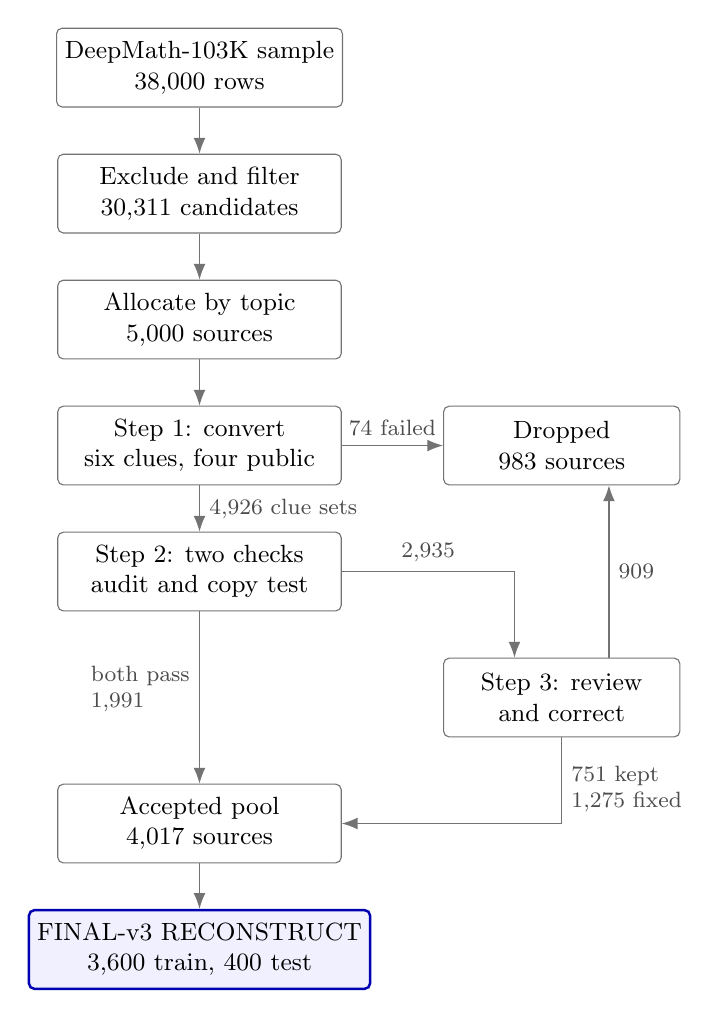
\begin{tikzpicture}[
  font=\small,
  box/.style={draw=black!55, rounded corners=2pt, minimum width=3.6cm, minimum height=1.0cm, align=center, inner sep=3pt},
  side/.style={box, minimum width=3.0cm},
  final/.style={box, draw=blue!70!black, line width=0.9pt, fill=blue!6},
  arr/.style={-{Latex[length=2mm]}, draw=black!55},
  lab/.style={font=\footnotesize, text=black!70, align=left}]
\node[box] (sample) at (0,0) {DeepMath-103K sample\\38,000 rows};
\node[box] (filter) at (0,-1.6) {Exclude and filter\\30,311 candidates};
\node[box] (alloc) at (0,-3.2) {Allocate by topic\\5,000 sources};
\node[box] (conv) at (0,-4.8) {Step 1: convert\\six clues, four public};
\node[box] (check) at (0,-6.4) {Step 2: two checks\\audit and copy test};
\node[box] (pool) at (0,-9.6) {Accepted pool\\4,017 sources};
\node[final] (final) at (0,-11.2) {FINAL-v3 RECONSTRUCT\\3,600 train, 400 test};
\node[side] (drop) at (4.6,-4.8) {Dropped\\983 sources};
\node[side] (fix) at (4.6,-8.0) {Step 3: review\\and correct};
\draw[arr] (sample) -- (filter);
\draw[arr] (filter) -- (alloc);
\draw[arr] (alloc) -- (conv);
\draw[arr] (conv) -- node[lab, right] {4,926 clue sets} (check);
\draw[arr] (check) -- node[lab, left, pos=0.45] {both pass\\1,991} (pool);
\draw[arr] (conv) -- node[lab, above] {74 failed} (drop);
\draw[arr] (check.east) -| node[lab, above, pos=0.25] {2,935} ([xshift=-0.6cm]fix.north);
\draw[arr] ([xshift=0.6cm]fix.north) -- node[lab, right] {909} ([xshift=0.6cm]drop.south);
\draw[arr] (fix.south) |- node[lab, right, pos=0.3] {751 kept\\1,275 fixed} (pool.east);
\draw[arr] (pool) -- (final);
\end{tikzpicture}}
\caption{RECONSTRUCT generation pipeline with source counts. Step 2 accepts a clue set only if both checks pass. Every other source gets one Step 3 call whose decision is final. The 983 dropped sources are 74 failed conversions, 486 sources judged unrepairable in Step 3, and 423 failed Step 3 calls.}
\label{fig:reconstruct-pipeline}
\end{figure}

\paragraph{Step 1: convert.} The converter sees the source question, answer, and DeepMath's first reference solution, which we treat as unverified. It either rejects the source or returns six ordered clues, each with a private note on where the source supports it. The first four clues are public and the last two are spares for Step 3. Two worked examples show the two ways to withhold information. One hides a premise that the student recovers from the answer, and the other hides which quantity is asked for.

\paragraph{Step 2: two independent checks.} A source-aware audit sees the source, reference solution, answer, and clues. It checks each clue, looks for a copied question, a disguised value, or a full solution, and must name the hidden element. A source-blind copy test sees only the answer and clues. It tries to rebuild a question by copying, paraphrasing, renaming, and reordering, without adding any new condition or target. A clue set passes only if the audit accepts it and the copy test cannot rebuild a question. Table~\ref{tab:recon-gate} shows that the copy test caught 496 clue sets that the audit had accepted.

\begin{table}[t]
\centering
\small
\setlength{\tabcolsep}{4pt}
\begin{tabular}{lr}
\toprule
Step 2 outcome & Sources \\
\midrule
Accepted by both checks & 1,991 \\
Rejected by both checks & 1,116 \\
Rejected by the copy test only & 496 \\
Rejected by the audit only & 433 \\
Rejected by one check, other call failed & 393 \\
Unresolved, a check call failed & 496 \\
Unresolved, audit asked for review & 1 \\
\midrule
All converted sources & 4,926 \\
\bottomrule
\end{tabular}
\caption{Step 2 outcomes for RECONSTRUCT. The copy test rejects a clue set when it can rebuild the question from the public text alone.}
\label{tab:recon-gate}
\end{table}


\paragraph{Step 3: review and correct.} Step 2 accepted only 1,991 sources, so each of the other 2,935 received one more call. It sees the source, the four clues, the two spares, and both Step 2 reviews. It can accept the clues unchanged, correct them, or mark the source unrepairable. A correction keeps every sound clue word for word and must remove a leak by withholding content, not by rewording it. The prompt rescued 9 of 40 training sources in a trial and was then applied unchanged. To limit cost, its decision is final. As an example of a caught leak, one source defines $a_1=1$ and $a_{n+1}=(1+a_1)\cdots(1+a_n)$. Its clue ``the recurrence implies $a_{n+1}=a_n(1+a_n)$'' holds at $n=1$ only if $a_1=1$, so it gave away the hidden starting value. The corrected clue adds ``for $n\ge2$''.

\subsection{Development trials}

We chose this design through small experiments on development sources that never enter the test set. A local 4-bit Qwen3-4B student was graded by DeepSeek. Table~\ref{tab:recon-dev} lists the main trials. A grounded success is a well-posed question with the supplied answer that uses every clue. A recovery additionally matches the original question. Fewer clues let more sources pass the checks without more recoveries, so we kept four. Removing the copy test admitted near-copies of the question, so we kept both checks. Changing prompt wording or the student's seed gave no reliable gain.

\begin{table}[t]
\centering
\footnotesize
\setlength{\tabcolsep}{3pt}
\begin{tabular}{>{\raggedright\arraybackslash}p{0.19\columnwidth}>{\raggedright\arraybackslash}p{0.37\columnwidth}>{\raggedright\arraybackslash}p{0.34\columnwidth}}
\toprule
Trial & Main change & Result \\
\midrule
First pilot & One to four clues per source & 3/8 and 1/12 grounded successes on two splits \\
Three clues & Show only the first three clues & 7/16 passed checks, 0 recoveries \\
Looser audit & Relax the leakage rule & 6/16 passed, 0/6 recoveries \\
Four clues & First four of six clues, both checks & 52/100 passed, mean score 44.4 \\
No copy test & Remove the source-blind check & at least 2/8 accepted near-copies \\
Correction & One review-and-correct call & 9/40 rejected sources rescued \\
\bottomrule
\end{tabular}
\caption{RECONSTRUCT development trials. Fewer clues let more sources pass but did not produce more recoveries.}
\label{tab:recon-dev}
\end{table}

\subsection{Final statistics}

The pipeline accepted 4,017 sources, and we kept 4,000 to match the topic and difficulty profile of the other tasks. All 400 test items come from base test sources that no development step used. The training split uses 3,197 base training sources and 403 base test sources that the test split did not need. Table~\ref{tab:recon-routes} gives the acceptance route of each kept item.

\begin{table}[t]
\centering
\small
\setlength{\tabcolsep}{3.5pt}
\begin{tabular}{lrrrr}
\toprule
Group & Step 2 & Fixed & Kept & Total \\
\midrule
Train & 1,780 & 1,152 & 668 & 3,600 \\
Test & 201 & 119 & 80 & 400 \\
\midrule
Algebra & 503 & 324 & 193 & 1,020 \\
Calculus & 540 & 324 & 160 & 1,024 \\
Discrete Math. & 404 & 320 & 238 & 962 \\
Number Theory & 534 & 303 & 157 & 994 \\
\midrule
Lower band & 1,553 & 784 & 448 & 2,785 \\
Upper band & 428 & 487 & 300 & 1,215 \\
\midrule
All & 1,981 & 1,271 & 748 & 4,000 \\
Share & 49.5\% & 31.8\% & 18.7\% & 100\% \\
\bottomrule
\end{tabular}
\caption{Acceptance route of the 4,000 kept RECONSTRUCT items. ``Step 2'' items passed both checks. ``Fixed'' items were corrected in Step 3 and ``Kept'' items were accepted unchanged in Step 3. The lower band is difficulty 5.0--6.5 and the upper band is 7.0--8.0.}
\label{tab:recon-routes}
\end{table}

Harder sources rely more on Step 3. It supplied 64.8\% of upper-band items but 44.2\% of lower-band items. The 1,271 corrected items changed 1,753 clues. Most corrections were small, with one clue changed in 877 items and two in 316. The recorded reasons were question disclosure in 1,296 changed clues, solution disclosure in 223, padding in 141, unsupported content in 76, and a disguised value in 11. Corrected items were not re-checked before inclusion. A later audit and copy test passed 508 of them, flagged 549, and has no result for 214. All 748 items accepted unchanged had been rejected or left unresolved by Step 2.

A kept clue has 15.4 words on average and a set of four clues has 61.6 words. The hidden questions have 33.1 words. The items cover 49 detailed topic paths with mean difficulty 6.21, and 47.3\% of the supplied answers are integers.

\subsection{Records and scoring}

The public record contains only the answer, the four clues, and the instruction. The private record holds the source question, acceptance route, Step 3 findings, and the original clues of corrected items. A source-aware grader checks whether the output keeps the source's premises and asks for the same quantity. A source-blind grader checks whether the new question is well formed, uses the clues, and is mathematically valid. Section~\ref{sec:eval} gives the scoring rule.

\section{Models and Training}

The student is Qwen3.5-2B and the teacher is Qwen3.8-27B. Both use text-only, non-thinking mode with bfloat16 weights. We checked all 248,070 shared token IDs and found identical token strings. Rendered prompts also matched token for token. This matters because the student and teacher probabilities must refer to the same next-token choices.

Every task run starts from a fresh student. LoRA adapters are applied to all attention and MLP projections with rank 64, scaling parameter $\alpha=64$, and dropout 0. Training has two stages. First, we perform supervised fine-tuning on teacher responses. Then we run reverse-KL on-policy distillation \citep{agarwal2024opd}.

\begin{table}[t]
\centering
\small
\setlength{\tabcolsep}{4pt}
\begin{tabular}{ll}
\toprule
Setting & Value \\
\midrule
Student and teacher & Qwen3.5-2B, Qwen3.8-27B \\
Adapter & LoRA rank 64, $\alpha=64$, dropout 0 \\
SFT data & 470 retained teacher responses \\
SFT optimization & 1 epoch, batch 16, 30 steps \\
SFT learning rate & $10^{-4}$ with cosine decay \\
OPD data & 16 steps $\times$ 32 new prompts \\
OPD learning rate & Constant $5\times10^{-5}$ \\
Rollout sampling & Temperature 1, top-$p$ 1 \\
\bottomrule
\end{tabular}
\caption{Training configuration shared by all three task-specific runs.}
\label{tab:training-settings}
\end{table}

For supervised fine-tuning, 512 questions per task are reserved for teacher-response generation and do not overlap evaluation or on-policy prompts. The teacher produces two samples per question at temperature 1.0, top-$p$ 1.0, and a 16,384-token limit. We keep the first completed sample that follows the required format and use the first 470 retained responses. The student trains for one epoch on response tokens only. Prompt tokens are masked. Batch size 16 gives 30 optimizer steps. AdamW uses learning rate $10^{-4}$, three warm-up steps, cosine decay to $10^{-5}$, weight decay 0, and gradient clipping at 1.0.

On-policy distillation starts from the supervised adapter and runs for 16 steps. Each step uses 32 distinct prompts and one current-student rollout per prompt, for 512 questions used once. Rollouts use temperature 1.0, top-$p$ 1.0, and a 16,384-token limit. At each generated token, the loss moves the student distribution toward the teacher distribution on the student's own response history. Importance weights are capped at 2.0. AdamW uses a constant learning rate of $5\times10^{-5}$, weight decay 0, and gradient clipping at 1.0. The adapter is synchronized with the generation server after every update.

\section{Evaluation and Baselines}
\label{sec:eval}

Each task has a fixed 400-question test set. JUDGE contains 200 correct and 200 incorrect proposed solutions. Generation uses temperature 1.0, top-$p$ 1.0, top-$k$ 0, one sample, seed 0, no presence or repetition penalty, and at most 32,768 new tokens.

SOLVE uses deterministic final-answer checks. JUDGE first parses the decision and error step, then uses a DeepSeek-V4.1-Flash rubric for the verdict, location, explanation, and mathematical validity. RECONSTRUCT uses a four-part rubric for source fidelity, task consistency, clue support, and mathematical validity. Each part is scored from 0 to 4, and the total is $6.25$ times their sum, out of 100. An output that only copies the answer or contains no question scores 0. Open-ended grading uses temperature 0 and low reasoning effort.

Table~\ref{tab:baseline} gives the zero-training baselines. The gap is largest on locating an error and reconstructing a supported question.

\begin{table}[t]
\centering
\small
\setlength{\tabcolsep}{4pt}
\begin{tabular}{lrr}
\toprule
Metric & Student & Teacher \\
\midrule
SOLVE accuracy & 55.8\% & 79.5\% \\
JUDGE verdict & 57.5\% & 73.5\% \\
JUDGE first wrong step & 18.0\% & 55.5\% \\
JUDGE rubric & 47.0 & 78.1 \\
RECONSTRUCT rubric & 33.5 & 70.1 \\
\bottomrule
\end{tabular}
\caption{Zero-training results. Rubric scores are out of 100. The first-wrong-step metric uses the 200 incorrect JUDGE items.}
\label{tab:baseline}
\end{table}

\section{Transfer Results}

Table~\ref{tab:transfer-main} reports the final checkpoint after supervised fine-tuning and on-policy distillation for each training task. Each parenthesized value is the paired change from the untrained student, followed by its 95\% bootstrap confidence interval. Detailed results for both stages appear in Appendix~\ref{app:transfer}.

\begin{table*}[t]
\centering
\footnotesize
\setlength{\tabcolsep}{5pt}
\begin{tabular}{lccc}
\toprule
Training data & SOLVE accuracy (\%) & JUDGE rubric (/100) & RECONSTRUCT (/100) \\
\midrule
None & 55.8 & 47.0 & 33.5 \\
SOLVE & 53.8 ($-2.0$ [$-7.2,+3.0$]) & 49.8 ($+2.9$ [$-0.4,+6.0$]) & 34.4 ($+1.1$ [$-2.3,+4.4$]) \\
JUDGE & 43.5 ($-12.2$ [$-18.0,-6.8$]) & 51.0 ($+4.0$ [$-0.1,+7.9$]) & 32.5 ($-0.6$ [$-4.3,+3.2$]) \\
RECONSTRUCT & 43.5 ($-12.2$ [$-17.5,-7.2$]) & 45.2 ($-1.9$ [$-5.3,+1.5$]) & 42.4 ($+8.7$ [$+5.5,+12.3$]) \\
\bottomrule
\end{tabular}
\caption{Transfer after training on one task form. Each trained row uses supervised fine-tuning followed by on-policy distillation. Parentheses contain the paired change from the untrained student and a 95\% bootstrap interval.}
\label{tab:transfer-main}
\end{table*}

RECONSTRUCT training produces the clearest same-task improvement. Its 8.7-point gain has an interval entirely above zero. JUDGE training improves the complete rubric by 4.0 points, but its interval includes a small negative value. The more direct first-wrong-step accuracy rises from 18.0\% to 28.0\%, a 10.0-point gain with a 95\% interval of $[+5.0,+15.0]$. Verdict accuracy changes from 57.5\% to 56.5\%, so the improvement comes from locating errors rather than making more binary decisions.

SOLVE training does not improve SOLVE accuracy over the untrained student. Supervised fine-tuning first reduces it to 48.5\%. On-policy distillation recovers part of this loss and reaches 53.8\%. JUDGE and RECONSTRUCT training both lower SOLVE accuracy to 43.5\%, and both confidence intervals exclude zero. Most other cross-task changes have intervals that include zero. The evidence therefore does not show broad transfer between the three forms.

The transfer is also asymmetric. RECONSTRUCT training improves RECONSTRUCT but lowers SOLVE. JUDGE training improves first-error identification but does not improve RECONSTRUCT. SOLVE training has small, uncertain changes on both other forms. This supports the main hypothesis that training form affects what the student learns, even when the mathematical topics and difficulty are controlled.

Output truncation is a concern for the JUDGE-trained checkpoint. Its cap rates are 13.8\% on SOLVE, 3.0\% on JUDGE, and 18.0\% on RECONSTRUCT. The corresponding rates for the SOLVE-trained checkpoint are 0.8\%, 0.0\%, and 3.8\%. For the RECONSTRUCT-trained checkpoint they are 4.0\%, 0.2\%, and 6.8\%. Some of the JUDGE-trained model's lower cross-task scores may therefore reflect unstable generation length as well as weaker reasoning.

\section{Limitations and Next Steps}

The JUDGE and RECONSTRUCT data are generated and checked by models. Independent checks reduce errors but do not replace a human audit. RECONSTRUCT has 549 corrected examples flagged by later checks and 214 without recorded follow-up checks. Teacher responses for supervised fine-tuning were selected for completion and format, not independently verified mathematical correctness.

The JUDGE release pool is nearly balanced by topic, difficulty, label, and error region, but step length still correlates with the label. The final production batch also uses v11 while earlier batches use v10. We will report results by step length and prompt batch. We will also audit a stratified sample across labels, topics, difficulties, error positions, and conversion paths.

RECONSTRUCT and part of JUDGE evaluation depend on model grading. These scores need calibration against human judgments. The transfer study currently uses one training run per task. The next stage will repeat the main comparisons with another seed, inspect truncated outputs, and test whether a mixture of task forms performs better than any single-task dataset.

\section{Conclusion}

We compare three ways of asking about the same mathematical subjects. The datasets use separate DeepMath questions and matched topic and difficulty distributions. The completed transfer results show useful improvement within RECONSTRUCT and in JUDGE error location, but little evidence that these improvements carry to the other forms. Training on JUDGE or RECONSTRUCT also lowers ordinary SOLVE accuracy. These results make question form a necessary experimental variable when distilling mathematical reasoning.

\bibliography{references}

\clearpage
\appendix

\section{Detailed Transfer Results}
\label{app:transfer}

Tables~\ref{tab:transfer-full} and~\ref{tab:transfer-secondary} give every reported checkpoint. SFT is supervised fine-tuning. OPD is the following on-policy distillation stage. JUDGE step accuracy is measured only on the 200 incorrect examples. Rubric scores can use fewer than 400 paired items because malformed or unscorable outputs are excluded.

\begin{table}[h]
\centering
\footnotesize
\setlength{\tabcolsep}{3pt}
\begin{tabular}{lrrr}
\toprule
Checkpoint & SOLVE & JUDGE & RECON. \\
\midrule
Untrained & 55.8 & 47.0 & 33.5 \\
SOLVE SFT & 48.5 & 43.7 & 32.6 \\
SOLVE SFT+OPD & 53.8 & 49.8 & 34.4 \\
JUDGE SFT & 39.0 & 46.4 & 29.8 \\
JUDGE SFT+OPD & 43.5 & 51.0 & 32.5 \\
RECON. SFT & 44.8 & 45.0 & 33.6 \\
RECON. SFT+OPD & 43.5 & 45.2 & 42.4 \\
\bottomrule
\end{tabular}
\caption{Primary checkpoint scores. JUDGE and RECONSTRUCT are rubric scores out of 100.}
\label{tab:transfer-full}
\end{table}

\begin{table}[h]
\centering
\footnotesize
\setlength{\tabcolsep}{2.7pt}
\begin{tabular}{lrrr}
\toprule
Checkpoint & Verdict & Step & Cap S/J/R \\
\midrule
Untrained & 57.5 & 18.0 & 0.0/0.0/0.2 \\
SOLVE SFT & 55.0 & 16.5 & 0.0/0.0/1.0 \\
SOLVE SFT+OPD & 56.0 & 19.5 & 0.8/0.0/3.8 \\
JUDGE SFT & 56.0 & 19.5 & 0.2/0.0/0.5 \\
JUDGE SFT+OPD & 56.5 & 28.0 & 13.8/3.0/18.0 \\
RECON. SFT & 54.8 & 15.5 & 0.0/0.0/0.5 \\
RECON. SFT+OPD & 56.8 & 13.0 & 4.0/0.2/6.8 \\
\bottomrule
\end{tabular}
\caption{Secondary JUDGE accuracies and output-cap rates. All values are percentages.}
\label{tab:transfer-secondary}
\end{table}

The paired changes that support the main conclusions are: JUDGE first wrong step, $+10.0$ [$+5.0,+15.0$], $n=200$; RECONSTRUCT after RECONSTRUCT training, $+8.7$ [$+5.5,+12.3$], $n=296$; SOLVE after JUDGE training, $-12.2$ [$-18.0,-6.8$], $n=400$; and SOLVE after RECONSTRUCT training, $-12.2$ [$-17.5,-7.2$], $n=400$.

Two unfiltered SOLVE warm-up checkpoints were also evaluated. SFT scored 43.5\% on SOLVE, 56.2\% on the JUDGE verdict, and 16.0\% on the first wrong step. SFT+OPD scored 52.2\%, 56.5\%, and 18.5\%. Their cap rates were 0.0/0.5/1.5\% and 2.0/0.2/5.0\%. These runs are diagnostic and are not used in the main matrix.

\begin{table}[h]
\centering
\footnotesize
\setlength{\tabcolsep}{2.4pt}
\begin{tabular}{lllr}
\toprule
Train & Test metric & Change [95\% CI] & $n$ \\
\midrule
SOLVE & SOLVE & $-2.0$ [$-7.2,+3.0$] & 400 \\
SOLVE & J verdict & $-1.5$ [$-4.5,+1.2$] & 400 \\
SOLVE & J step & $+1.5$ [$-1.5,+5.0$] & 200 \\
SOLVE & J rubric & $+2.9$ [$-0.4,+6.0$] & 394 \\
SOLVE & RECON. & $+1.1$ [$-2.3,+4.4$] & 296 \\
\midrule
JUDGE & SOLVE & $-12.2$ [$-18.0,-6.8$] & 400 \\
JUDGE & J verdict & $-1.0$ [$-5.5,+3.5$] & 400 \\
JUDGE & J step & $+10.0$ [$+5.0,+15.0$] & 200 \\
JUDGE & J rubric & $+4.0$ [$-0.1,+7.9$] & 393 \\
JUDGE & RECON. & $-0.6$ [$-4.3,+3.2$] & 267 \\
\midrule
RECON. & SOLVE & $-12.2$ [$-17.5,-7.2$] & 400 \\
RECON. & J verdict & $-0.8$ [$-3.5,+1.8$] & 400 \\
RECON. & J step & $-5.0$ [$-9.5,-1.0$] & 200 \\
RECON. & J rubric & $-1.9$ [$-5.3,+1.5$] & 393 \\
RECON. & RECON. & $+8.7$ [$+5.5,+12.3$] & 296 \\
\bottomrule
\end{tabular}
\caption{Paired changes for the final SFT+OPD checkpoints. J denotes JUDGE.}
\label{tab:transfer-final-full}
\end{table}

\clearpage
\section{Final Prompt Record}
\label{app:prompts}

This appendix records the task instructions needed to interpret the reported data and scores. The final submission will add public archival links for the full generation and grading prompts. No local directory paths are used here.

\paragraph{SOLVE student instruction.}
The model receives one mathematics problem. It must give a complete and mathematically correct derivation, include the equations and intermediate calculations needed to verify the result, avoid exploratory or repetitive text, and end with exactly one \texttt{<final\_answer>} tag containing only the final answer.

\paragraph{JUDGE student instruction.}
The model receives a problem and a numbered proposed solution. It must check the steps in order, decide whether the solution is correct, and return three fields: \texttt{Decision}, \texttt{First wrong step}, and \texttt{Explanation}. If the proposal is incorrect, the step must be the earliest mathematical error. If it is correct, the first wrong step is \texttt{none}. The model must not judge only from the final answer or continue a different solution.

\paragraph{JUDGE generation instruction.}
The final generator first checks that the source question, answer, and reference solution are consistent. It may return \texttt{NOT\_SUITABLE}. Otherwise it produces five to eight numbered mathematical steps in JSON. A correct item must be valid throughout. An incorrect item must introduce one natural first error at any substantive step while keeping all previous steps correct. The final batch prefers seven or eight steps only when the source solution naturally supports that length. The output also contains the private verdict, first-error step, concise explanation, and source-specific error label. Three examples show a correct trace, a propagated algebraic error, and an error in applying a theorem.

\paragraph{RECONSTRUCT student instruction.}
The model receives a supplied answer and four clues from a hidden mathematics problem. It must write one complete, mathematically meaningful question supported by those clues and explain why the supplied answer is valid for that question. It may produce a valid alternative to the hidden source because the clues can leave more than one possible reconstruction. It must not claim that unstated information was given.

\paragraph{RECONSTRUCT generation instruction.}
The generator sees the source question, answer, and an unverified reference solution. It may reject the source or produce six concise clues. Four are public and two are reserved for correction. The public clues must contain enough connected mathematical evidence for a valid reconstruction, omit at least one essential part of the original specification, and avoid copying or closely paraphrasing the hidden question or full solution.

\paragraph{Grading prompts.}
The JUDGE grader scores the verdict, first-error location, explanation, and mathematical validity. The RECONSTRUCT source-aware grader scores fidelity to the source mathematics and task type. The source-blind grader checks whether the new problem is well formed, supported by the four clues, and mathematically valid. These graders receive structured outputs so that malformed responses can be separated from mathematical errors.

\end{document}
